\section{Identification du sens du résultat}


\subsection{Contexte}

\begin{frame}[t]{\mysubsectiontitle}
	Restriction du problème d'identification des demandes
\begin{itemize}	\small
	\item Uniquement les décisions à une demande de la catégorie
	\begin{itemize}\scriptsize
		\item Raison: plus de $50\%$ des documents dans la majorité des catégories
	\end{itemize}
	\item Classification binaire (éviter les subtilités de rédaction)
	\begin{itemize} \scriptsize
		\item Raison: les demandes sont en majorité \textbf{acceptées} ou \textbf{rejetées}
	\end{itemize}
\end{itemize}
\centering 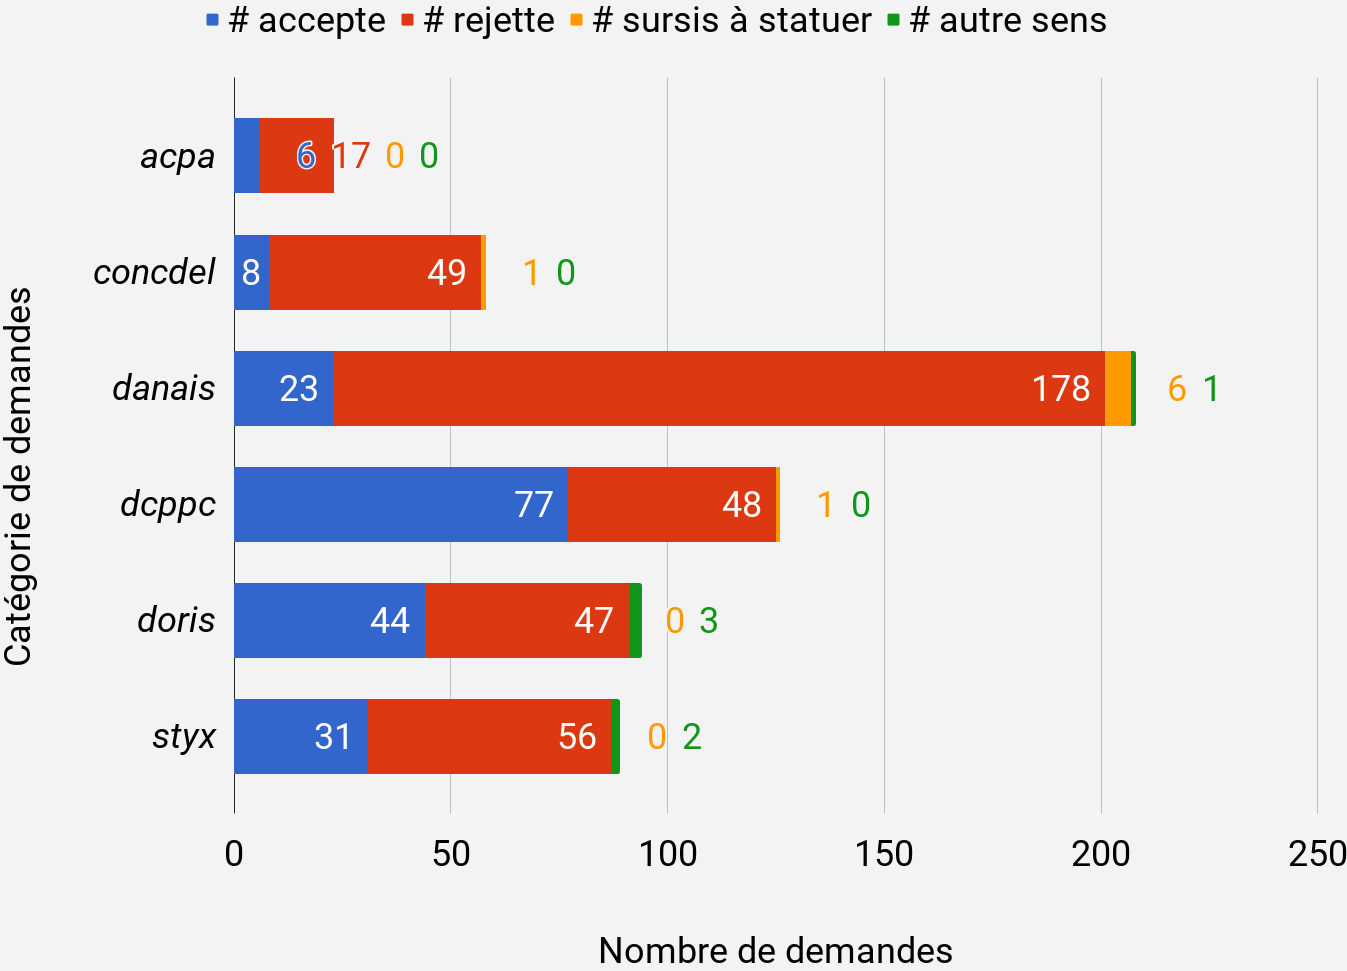
\includegraphics[width=0.7\textwidth]{chartDistrSens.png}
\end{frame}

\begin{frame}[t]{\mysubsectiontitle}
	Plusieurs algorithmes classiques existent
	\begin{itemize} \small
		\item Classifieur bayésien naïf \cite{duda1973patternclass} 
		\item K-plus-proches-voisins \cite{cover1967knn}
		\item SVM \cite{vapnik1995statlearning}
		\item Arbre de décision
		\item Analyse discriminante linéaire \cite{fisher1936linearDA} et quadratique \cite{McLachlan1992DiscrAnalyStatPattRecog-QDA}
		\item NBSVM \cite{wang2012nbsvm}
		\item fastText \cite{grave2017fasttextcls}
		\item etc.	
	\end{itemize}
\end{frame}


\subsection{Méthode proposée : adaptations de la régression Gini-PLS}

\begin{frame}[t]{\mysubsectiontitle}
Régression	Gini-PLS
\begin{itemize}\small
	\item PLS \cite{wold1966pls} (régression partielle des moindres carrés) 
	\begin{itemize}\scriptsize
		\item Réduction supervisée de dimensions $x_1, x_2, ..., x_m$ en composantes orthogonales $t_1, ...., t_h$
		
		\[t_h = \sum_{k=1}^m w_{hk}\cdot \hat{U}_{(h-1)k}\] 
		
		avec $\hat{U}_{0k} = x_{k}$, $\forall h > 0, \hat{U}_{hk}$ est le résidu de la régression de $x_k$ sur $t_1, ..., t_{h-1}$ ()
		
		et $w_{hj} = \frac{cov(\varepsilon_h, \hat{U}_{(h-1)j})}{\sqrt{\sum_{j=1}^m cov^2(\varepsilon_h, \hat{U}_{(h-1)j})}}$
		\item Régression de $y$ dans l'espace réduit
		\[y=c_1 t_1 + ... + c_h t_h + \varepsilon_h\]			
		%\item intérêt : robustesse au problème de haute dimension et élimination du pro
	\end{itemize}
	\item Gini-PLS  \cite{mussard2018ginipls}
	\begin{itemize} \scriptsize
		\item Remplacement de la covariance $cov(x_j, y)$ par la covariance de Gini $cog(y; x_j) := cov(y; R(x_j))$
		\item 
	\end{itemize}	 	
	
\end{itemize} 
\end{frame}

\begin{frame}[t]{\mysubsectiontitle}
\begin{enumerate}
\setlength\itemsep{1.5em}

\item Gini-PLS généralisé
\begin{itemize}
	\item Utilisation de l'opérateur co-Gini généralisé : $cog_\nu(x_\ell,x_k) := -\nu cov(x_\ell,r_{k}^{\nu-1}) ; \ \nu > 1$
\end{itemize}
 pous disposer d'un curseur $\nu$ permettant de régler le compromis entre l'atténuation de la variabilité des variables et l'influence des queues de distributions de ces variables

\item Logit-PLS:  $\forall j > 1$, les $w_{hj} $ sont les coefficients de la régression logistique de $y$ sur les composantes $t_1, ..., t_{h-1}, u_{(h-1)j}$ \cite{tenenhaus2005logitpls}

\item Gini-Logit-PLS: covariance Gini pour $u_{(h)j}$ et coefficient Logit pour les $w_{hj}$
\end{enumerate}
\end{frame}


\subsection{Résultats expérimentaux}

%\begin{frame}[t]{\mysubsectiontitle}
%	Résultats obtenus avec fastText et NBSVM
%	\begin{table}[htb]
%		\scriptsize
%		\begin{center}
%			\begin{tabular}{|c|c|c|c|c|c|c|c|c|}
%				\hline
%				Cat. Dmd. & Algo. & {Préc.} & {Préc. équi.} & {err-0} & {err-1} & $F_1(0)$ & $F_1(1)$ & {$F_{1macro}$} \\ \hline
%				\textit{dcppc} & NBSVM & 0.875 & 0.812 & 0 & 0.375 & 0.916 & 0.752 & \textbf{0.834} \\ \hline
%				\textit{danais} & fastText & 0.888 & 0.5 & 0 & 1 & 0.941 & 0 & 0.47 \\ \hline
%				\textit{danais} & NBSVM & 0.888 & 0.5 & 0 & 1 & 0.941 & 0 & 0.47 \\ \hline
%				\textit{concdel} & fastText & 0.775 & 0.5 & 0 & 1 & 0.853 & 0 & 0.437 \\ \hline
%				\textit{concdel} & NBSVM & 0.775 & 0.5 & 0 & 1 & 0.873 & 0 & 0.437 \\ \hline
%				\textit{acpa} & fastText & 0.745 & 0.5 & 0 & 1 & 0.853 & 0 & 0.426 \\ \hline
%				\textit{acpa} & NBSVM & 0.745 & 0.5 & 0 & 1 & 0.853 & 0 & 0.426 \\ \hline
%				\textit{doris} & NBSVM & 0.5 & 0.492 & 0.167 & 0.85 & 0.63 & 0.174 & 0.402 \\ \hline
%				\textit{dcppc} & fastText & 0.667 & 0.5 & 0 & 1 & 0.8 & 0 & 0.4 \\ \hline
%				\textit{styx} & fastText & 0.667 & 0.5 & 0 & 1 & 0.8 & 0 & 0.4 \\ \hline
%				\textit{styx} & NBSVM & 0.667 & 0.5 & 0 & 1 & 0.8 & 0 & 0.4 \\ \hline
%				\textit{doris} & fastText & 0.523 & 0.5 & 0 & 1 & 0.686 & 0 & 0.343 \\ \hline
%			\end{tabular}
%		\end{center}
%		0 = "rejette" et 1 == "accepte"
%	\end{table}
%	\scriptsize
%	\textbf{Influence du déséquilibre et de la (très) faible taille des données}
%\end{frame}

\begin{frame}[t]{\mysubsectiontitle}
	Comaparaison des classifieurs PLS aux classifieurs classiques

	\scriptsize
	\centering
	\begin{tabular}{|l|l|l|l|l|}
		\hline
		\textbf{Représentation} & \textbf{Algorithme} & \textbf{$F_{1}$} & $F_{1_\text{arbre}} - F_1$ & \textbf{$F_{1_\text{max}} - F_{1_\text{min}}$} \\ \hline
		
		$tf-gss$ & Arbre & 0.668 & 0 & 0.42\\ \hline
		$tf - avg_{global}$ & LogitPLS & 0.648 & 0.02 & 0.263  \\ \hline
		$tf - avg_{global}$ & StandardPLS & 0.636 & 0.032 & 0.346 \\ \hline
		$tf - \Delta_{DF}$ & GiniPLS & 0.586 & 0.082 & 0.426 \\ \hline
		$tf - \Delta_{DF}$ & GiniLogitPLS & 0.578 & 0.09 & 0.547 \\ \hline
		- & NBSVM & 0.494 & 0.174 & 0.434  \\ \hline
		- & fastText & 0.412 & 0.256 & 0.127 \\ \hline
	\end{tabular}	

\end{frame}

\begin{frame}[t]{\mysubsectiontitle}
	Amélioration de la classification par restriction du document

	\tiny
	\centering
	
	\begin{tabular}{|c|l|l|l|c|}
		\hline
		{Catégorie} & \multicolumn{1}{c|}{Zone} & \multicolumn{1}{c|}{Représentation} & \multicolumn{1}{c|}{Algorithme} & $F_1$ \\ \hline
		\multirow{3}{*}{\textit{acpa}} & \textbf{demande\_resultat\_a\_resultat\_context} & $tf-dbidf$ & \textbf{Arbre} & \textbf{0.846} \\ 
		& litige\_motifs\_dispositif & $tf-dbidf$ & StandardPLS & 0.697 \\ 
		& litige\_motifs\_dispositif & $tf-avg_{global}$ & LogitPLS & 0.683 \\ \hline
		
		\multirow{3}{*}{\textit{concdel}} & \textbf{litige\_motifs\_dispositif} & \textbf{$tf-gss$} & \textbf{Arbre} & \textbf{0.798} \\ 
		& motifs & $tf-idf$ & GiniLogitPLS & 0.703 \\ 
		& context & $logave-dbidf$ & StandardPLS & 0.657 \\ \hline
		
		\multirow{3}{*}{\textit{danais}} & \textbf{demande\_resultat\_a\_resultat\_context} & \textbf{$avg_{local}-\chi^2$} & \textbf{Arbre} & \textbf{0.813} \\ 
		& demande\_resultat\_a\_resultat\_context & $atf-avg_{global}$ & LogitPLS & 0.721 \\ 
		& demande\_resultat\_a\_resultat\_context & $atf-avg_{global}$ & StandardPLS & 0.695 \\ \hline
		
		\multirow{3}{*}{\textit{dcppc}} & \textbf{demande\_resultat\_a\_resultat\_context} & $tf-\chi^2$ & \textbf{Arbre} & \textbf{0.985} \\ 
		& demande\_resultat\_a\_resultat\_context & $tf-\chi^2$& LogitPLS & 0.94 \\ 
		& litige\_motifs\_dispositif & $tp-mar$ & StandardPLS & 0.934 \\ \hline
		
		\multirow{3}{*}{\textit{doris}} & \textbf{litige\_motifs\_dispositif} & $tp-dsidf$ & \textbf{GiniPLS} & \textbf{0.806} \\
		& litige\_motifs\_dispositif & $tp-dsidf$ & GiniLogitPLS & 0.806 \\
		& litige\_motifs\_dispositif & $atf-ig$ & StandardPLS & 0.772 \\ \hline
		
		\multirow{3}{*}{\textit{styx}} & \textbf{motifs} & $tf-dsidf$ & \textbf{Arbre} & \textbf{1} \\ 
		& demande\_resultat\_a\_resultat\_context & $logave-dsidf$ & GiniLogitPLS & 0.917 \\ 
		& litige\_motifs\_dispositif & $tf-rf$& GiniPLS & 0.833 \\ \hline
	\end{tabular}
	
\end{frame}